\documentclass[aspectratio=169,11pt]{beamer} % slides at 16:9, the shape of most screens and projectors
% Beamer loads hyperref itself and spaces its own paragraphs, so neither hyperref nor parskip is loaded here

% References
\usepackage{csquotes}                   % quotation marks that follow the document's language
\usepackage[backend=biber,style=apa,natbib=true]{biblatex} % APA 7; compile with Biber
\DeclareLanguageMapping{australian}{british-apa}
\usepackage{xurl} % allow long bibliography URLs to wrap within the page
\addbibresource{references.bib}

% Look
\usetheme{Madrid}                       % a built-in theme: coloured title bars, and author, title and page number along the bottom
% \usecolortheme{seahorse}              % uncomment for softer colours; try dolphin or whale too
\setbeamertemplate{navigation symbols}{} % hide the small navigation icons in the corner
\usepackage[australian]{babel}          % Australian hyphenation, and \today as 17 October 2026
\usepackage{iftex}                      % tells which TeX engine is running
\ifPDFTeX                               % for pdfLaTeX only:
  \usepackage[T1]{fontenc}              % proper accented letters, and text that copies cleanly from the PDF
  \usepackage{lmodern}                  % Latin Modern, a crisp scalable version of the default font
\fi                                     % XeLaTeX, LuaLaTeX and Tectonic already use Unicode fonts, which print a typed ’ or é as it is

% Maths
\usepackage{amsmath}                    % align, cases, matrices and \text inside maths

% Figures
\usepackage{pgfplots}                   % charts drawn from data, right in the slides
\pgfplotsset{compat=1.18}               % use current pgfplots behaviour (label placement and so on)

% Code
\usepackage{listings}                   % code with coloured keywords; a frame holding code needs [fragile]
\lstset{                                % how code looks: Python, keywords bold, comments grey
  language=Python,
  basicstyle=\ttfamily\small,
  keywordstyle=\color{blue!60!black}\bfseries,
  commentstyle=\color{gray},
  stringstyle=\color{teal},
  columns=fullflexible, keepspaces,     % natural letter spacing, indents kept
  showstringspaces=false
}

% Links: Beamer passes the title and author to the PDF itself
\hypersetup{                            % details shown in the PDF viewer’s document properties
  pdfsubject = {Comparing insertion sort and merge sort},
  pdflang    = {en-AU}
}

\title{Why merge sort wins}
\subtitle{Counting comparisons in two sorting algorithms}
\author{Your Name}
\institute[Your University]{School of Computing, Your University} % [short form] for the footer
\date{\today}

\begin{document}

\begin{frame}
  \titlepage
\end{frame}

\begin{frame}{Outline}
  \tableofcontents
\end{frame}

\section{The problem}

\begin{frame}{Sorting is everywhere}
  \begin{itemize}
    \item Search results, inboxes and leaderboards are all sorted lists.
    \pause
    \item A slow sort is fine for ten items and hopeless for ten million.
    \pause
    \item The question for today: \alert{how does the work grow with the list?}
  \end{itemize}
\end{frame}

\section{Two algorithms}

\begin{frame}[fragile]{Insertion sort}
  Take each item in turn and slide it left until it's in place.
\begin{lstlisting}
def insertion_sort(items):
    for i in range(1, len(items)):
        current = items[i]
        j = i - 1
        while j >= 0 and items[j] > current:
            items[j + 1] = items[j]  # shift the bigger item right
            j -= 1
        items[j + 1] = current
    return items
\end{lstlisting}
\end{frame}

\begin{frame}{How much work is insertion sort?}
  In the worst case (a list in reverse order) item $i$ is compared with all $i$ items before it:
  \begin{equation*}
    C(n) = \sum_{i=1}^{n-1} i = \frac{n(n-1)}{2}.
  \end{equation*}
  \begin{block}{In short}
    Doubling the list roughly \alert{quadruples} the work: $C(n)$ grows like $n^2$.
  \end{block}
\end{frame}

\begin{frame}[fragile]{Merge sort}
  \begin{columns}[T]
    \begin{column}{0.55\textwidth}
\begin{lstlisting}
def merge_sort(items):
    if len(items) <= 1:
        return items
    middle = len(items) // 2
    left = merge_sort(items[:middle])
    right = merge_sort(items[middle:])
    return merge(left, right)
\end{lstlisting}
    \end{column}
    \begin{column}{0.4\textwidth}
      Halve the list, sort each half, then merge them in one pass:
      \begin{align*}
        T(1) &= 0, \\
        T(n) &= 2\,T(n/2) + n.
      \end{align*}
      For $n$ a power of two this solves to $T(n) = n \log_2 n$.
    \end{column}
  \end{columns}
\end{frame}

\section{Measuring them}

\begin{frame}{Comparisons as the list grows}
  \centering
  \begin{tikzpicture}
    \begin{axis}[
        width=0.8\textwidth, height=0.6\textheight,
        xlabel={Items in the list, $n$}, ylabel={Comparisons},
        xmin=0, xmax=100, ymin=0,
        legend pos=north west, legend cell align=left,
      ]
      \addplot[very thick, red!70!black, domain=1:100, samples=50] {x*(x-1)/2};
      \addlegendentry{Insertion sort, $n(n-1)/2$}
      \addplot[very thick, teal, domain=1:100, samples=50] {x*ln(x)/ln(2)};
      \addlegendentry{Merge sort, $n \log_2 n$}
    \end{axis}
  \end{tikzpicture}
\end{frame}

\begin{frame}{Take-aways}
  \begin{itemize}
    \item Insertion sort does about $n^2/2$ comparisons; merge sort about $n \log_2 n$.
    \item At $n = 100$ that's 4,950 against 664; at a million items, hours against seconds.
    \item Insertion sort still wins on short or nearly sorted lists, which is why real libraries use both.
  \end{itemize}
  \vfill
  \centering
  \Large Questions?
\end{frame}

\begin{frame}[allowframebreaks]{References}
\printbibliography[heading=none]
\end{frame}

\end{document}
